% !TEX root = ./main.tex
% Translating into Intermediate Code
% ======================================================

\begin{figure}[H]
    \centering
    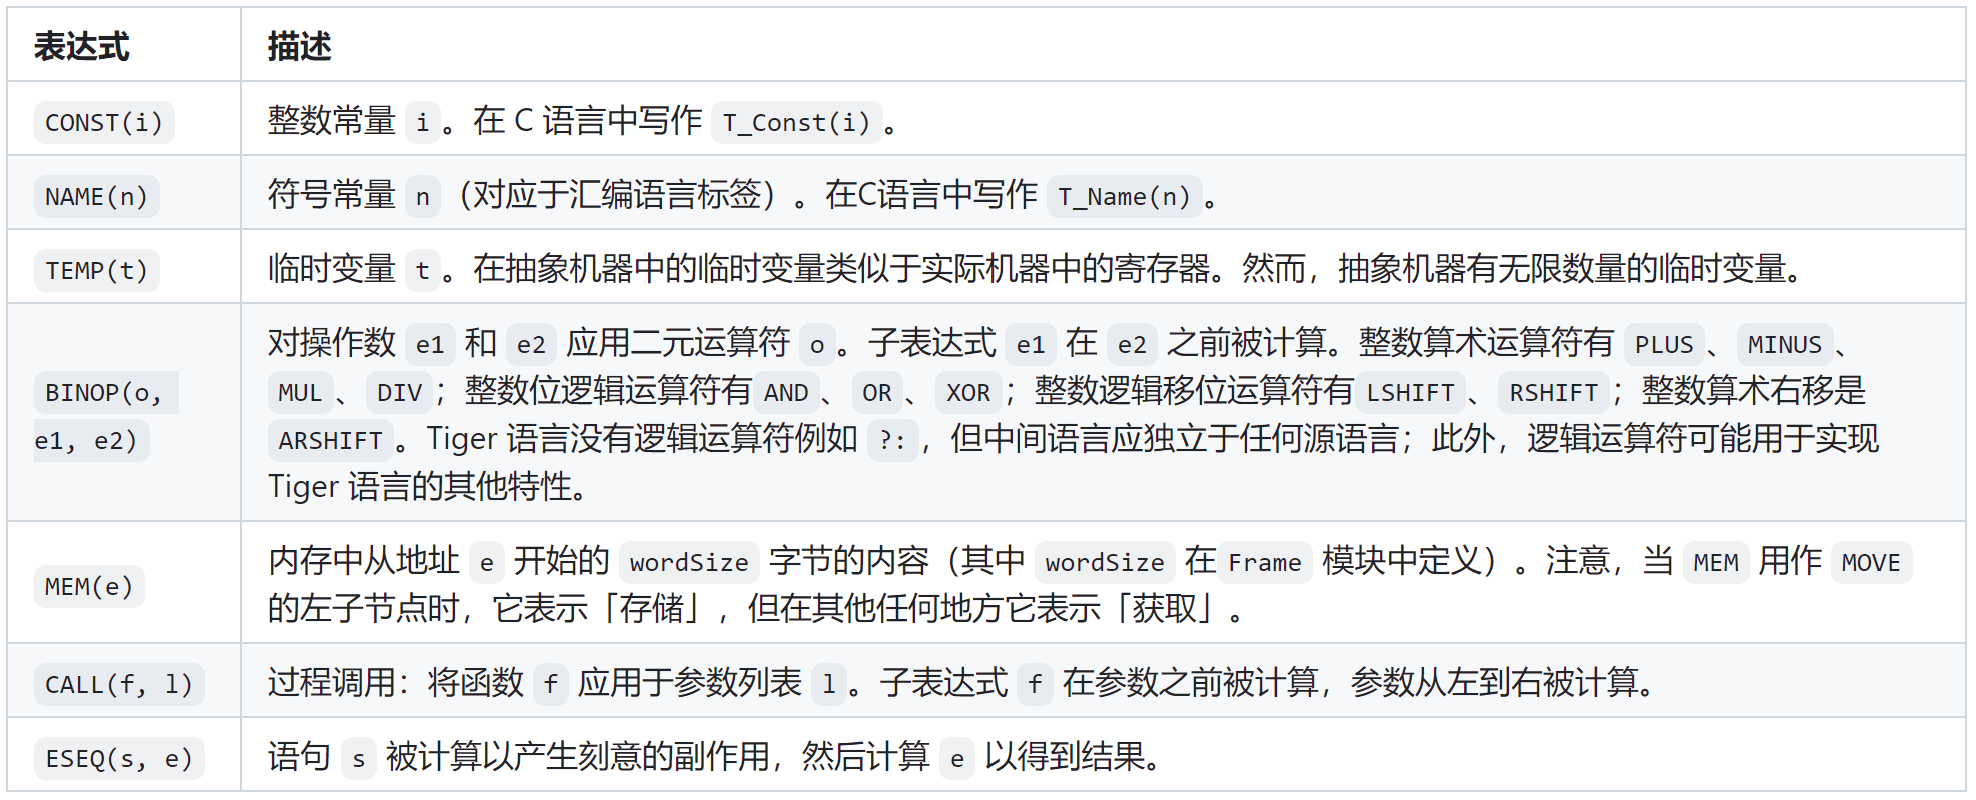
\includegraphics[width=\linewidth]{figures/ir2.png}
\end{figure}

\begin{figure}[H]
    \centering
    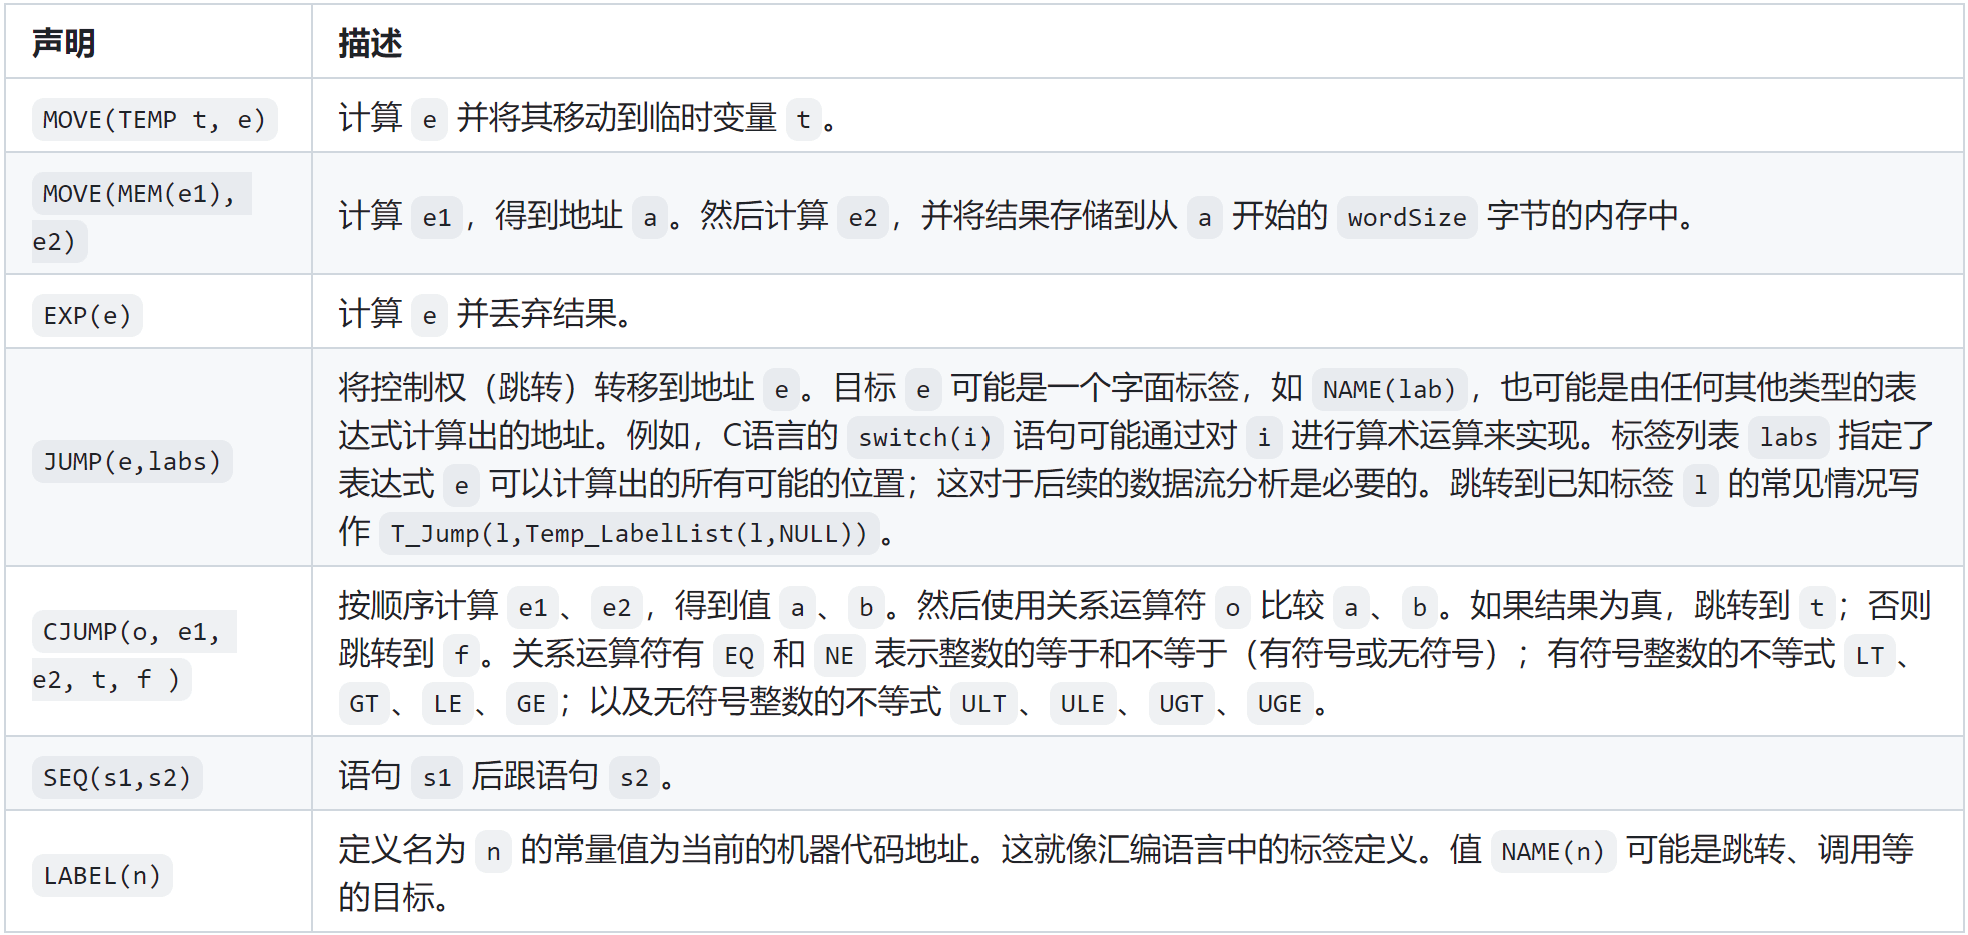
\includegraphics[width=\linewidth]{figures/ir1.png}
\end{figure}

\par \noindent 函数调用:\texttt{CALL(NAME lf , [sl, e1, e2, . . . , en])},其中 \texttt{lf} 是函数标签,
\texttt{sl} 是 static link,\texttt{e1, e2, . . . , en} 是参数。函数被翻译为 prologue、body 和 epilogue 三部分,
prologue = 
1. 声明一个函数开始的伪指令;
2. 函数名 label 的定义;
3. 调整栈指针、分配新的栈帧;
4. 将逃逸(escaping)参数保存至栈帧、将非逃逸参数传送到新临时寄存器;
5. 保存此函数用到的 callee-save 寄存器(包括返回地址寄存器)。
body = 函数体。
epilogue =
1. 保存返回值;
2. 恢复 callee-save 寄存器;
3. 恢复栈指针、释放栈帧;
4. 返回指令;
5. 声明函数结束的伪指令。


% ======================================================
% reference: https://cubicy.icu/compiler-construction-principles/#Part-13-%E4%B8%AD%E9%97%B4%E8%A1%A8%E7%A4%BA-IR
% ======================================================